\chapter{Software Architecture Design}
\label{ch:software-architecture-design}

This chapter describes the software architecture design of the EEG-based Motor Imagery (MI) classification system using Self-Supervised Learning (SSL). The system is designed to support research workflows, including dataset integration, preprocessing, SSL model training, evaluation, and visualization. Unified Modeling Language (UML) diagrams are used to represent structural and behavioral aspects of the system architecture.

\section{Domain Model}
\label{sec:domain-model}

The domain model captures core research entities and their relationships in the context of EEG analysis and SSL-based classification. These entities are grounded in scientific workflows rather than business operations.

\begin{itemize}
    \item \textbf{EEGDataset:} Represents structured EEG data collected from experiments, including metadata and raw signals.
    \item \textbf{Preprocessor:} Responsible for applying signal filtering, artifact removal, and standardization.
    \item \textbf{SSLModel:} Represents the core self-supervised learning module, including its architecture and training process.
    \item \textbf{EvaluationReport:} Contains metrics (accuracy, F1-score, ROC-AUC) derived from model evaluation.
    \item \textbf{Researcher:} A user interacting with the system to upload data, configure models, and interpret results.
\end{itemize}

\begin{figure}[H]
    \centering
    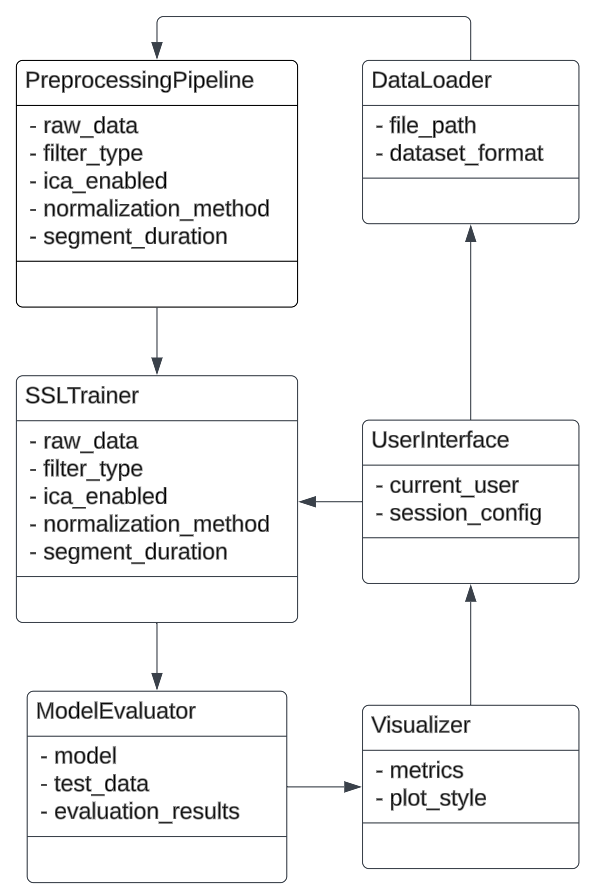
\includegraphics[width=0.75\textwidth]{domain-model-eeg.png}
    \caption{Domain Model for EEG SSL Research Framework}
    \label{fig:figure9}
\end{figure}

\section{Design Class Diagram}
\label{sec:design-class-diagram}

The class diagram provides a technical breakdown of system components. Classes are grouped by functionality into modules such as Data Handling, Model Training, and Evaluation.

\begin{itemize}
    \item \textbf{DataLoader:} Loads EEG datasets and parses metadata.
    \item \textbf{PreprocessingPipeline:} Applies band-pass filters, ICA, normalization, and data segmentation.
    \item \textbf{SSLTrainer:} Implements self-supervised learning algorithms and manages training sessions.
    \item \textbf{ModelEvaluator:} Validates model outputs, computes evaluation metrics, and stores performance data.
    \item \textbf{Visualizer:} Displays results through plots and summaries for analysis.
    \item \textbf{UserInterface:} Connects researchers with backend components for configuring and visualizing workflows.
\end{itemize}

\begin{figure}[H]
    \centering
    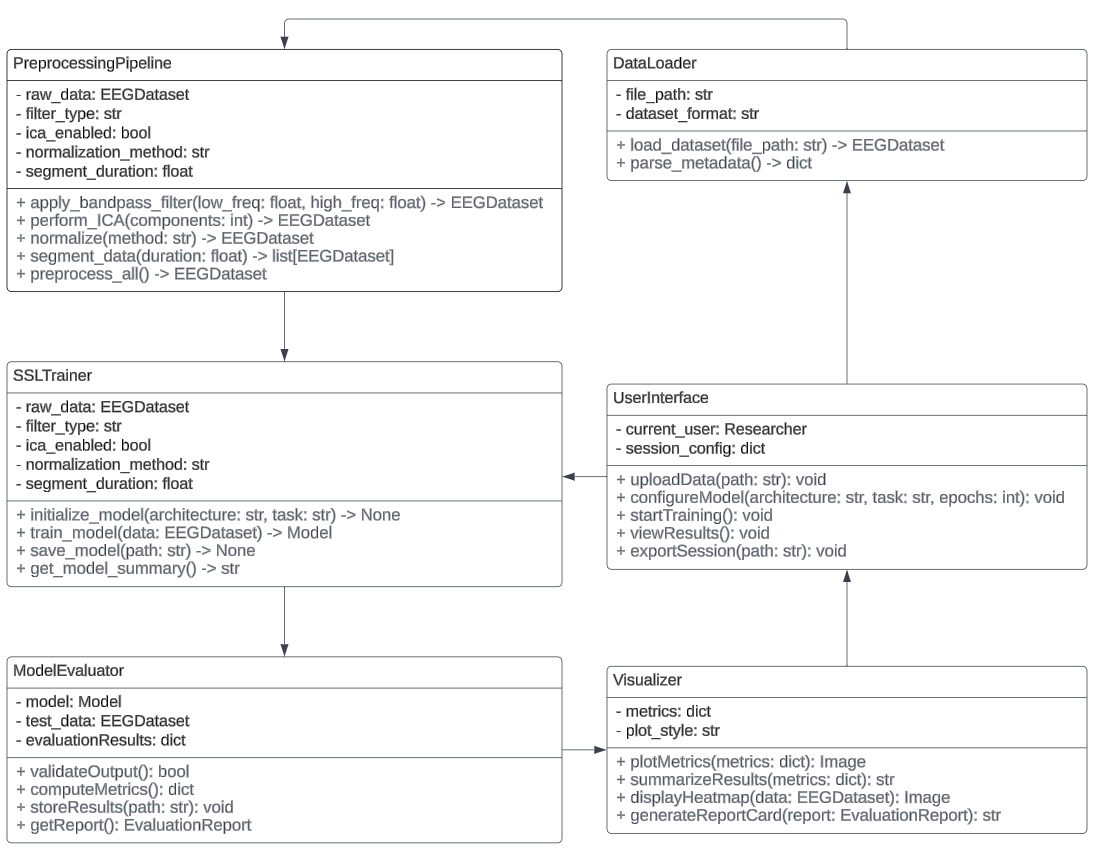
\includegraphics[width=0.95\textwidth]{design-class-diagram-eeg.png}
    \caption{Design Class Diagram for EEG SSL System}
    \label{fig:figure7}
\end{figure}

\section{Sequence Diagram}
\label{sec:sequence-diagram}

The following sequence diagram illustrates the typical interaction for training a new SSL model on a selected EEG dataset:

\textbf{Scenario: SSL Model Training Workflow}
\begin{enumerate}
    \item Researcher selects and uploads EEG data.
    \item The system applies preprocessing to the dataset.
    \item SSL model is initialized with pretext task configurations.
    \item Training begins, and progress is logged.
    \item Evaluation metrics are computed and visualized.
\end{enumerate}

\begin{figure}[H]
    \centering
    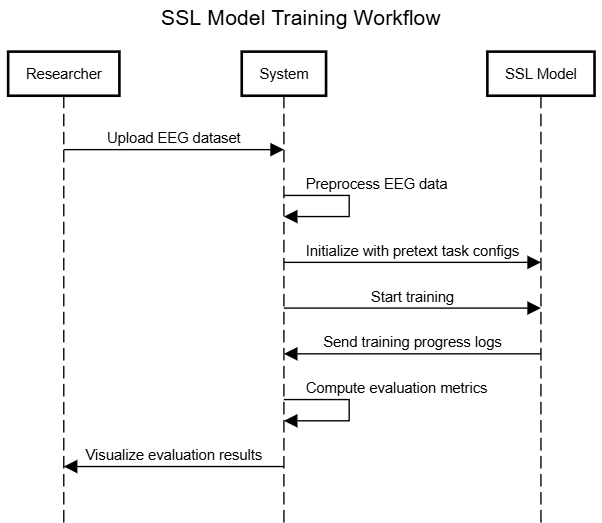
\includegraphics[width=0.9\textwidth]{figures/sequence-diagram-ssl-eeg}
    \caption{Sequence Diagram – SSL Model Training Flow}
    \label{fig:figure8}
\end{figure}

\section{Algorithm}
\label{sec:algorithm}

The following pseudocode outlines the simplified self-supervised learning training loop used in the project.
It includes feature transformation, encoding, and contrastive loss calculation.

\begin{verbatim}
Algorithm 1: Self-Supervised EEG Feature Learning
Input: Unlabeled EEG samples X
Output: Learned representations Z

for epoch in range(num_epochs):
    for batch in X:
        x1, x2 = Augment(batch)
        z1 = Encoder(x1)
        z2 = Encoder(x2)
        loss = ContrastiveLoss(z1, z2)
        UpdateWeights(loss)
\end{verbatim}

\section{AI Component}
\label{sec:ai-component}

The AI module in this system is built around a Self-Supervised Learning framework based on a dual-view contrastive encoder architecture.
It supports flexible pretext tasks and multiple EEG datasets.

\begin{itemize}
    \item \textbf{Encoder Network:} A convolutional network tailored to EEG signal structures (e.g., EEGNet or custom CNNs).
    \item \textbf{Pretext Tasks:}
    \begin{itemize}
        \item Spectral Band Masking
        \item Temporal Shuffling
        \item Channel Dropout
    \end{itemize}
    \item \textbf{Loss Function:} InfoNCE or triplet contrastive loss adapted to time-series EEG embeddings.
    \item \textbf{Fine-tuning Strategy:} Optionally transfers learned representations to downstream MI classification using supervised labels.
\end{itemize}

